\chapter{Einleitung}

Das \ac{RL} kann als zielorientierte Interaktion eines lernenden Subjekts mit seiner Umgebung beschrieben werden. Zusammen mit dem Supervised und Unsupervised Lernen bildet es die drei großen Paradigmen des maschinellen Lernens. Während bei den beiden Erstgenannten für gewöhnlich ein feststehender Datensatz die Basis des Lernprozesses bildet, gibt es diesen im \ac{RL} nicht. Stattdessen wird durch die Interaktion mit der Umgebung gelernt. Mittels \ac{RL} konnten in den vergangenen Jahren verschiedenste Problemstellungen erfolgreich gemeistert werden. Diese Erstrecken sich über Themen der Robotik \cite{MappingPlanning}, über das Spielen von Brettspielen wie Go \cite{Go}, bis hin zum Lösen algorithmischer Probleme \cite{DNC}. In vielen Bereichen konnten die Ergebnisse mittels \ac{RL} wahlweise signifikant verbessert werden oder überhaupt erst ermöglicht werden. Aufgrund der vielfältigen Einsatzmöglichkeiten und erzielten Resultate ist das \ac{RL} ein Thema von großem Interesse in der aktuellen Forschung im Bereich des maschinellen Lernens.

Das lernende Subjekt wird als Agent bezeichnet. Dieser befindet sich in einer Umgebung und wird in selbiger mit einer Problemstellung konfrontiert. So kann er sich beispielsweise in einem Labyrinth befinden und soll den Weg hinaus finden. Dazu stehen dem Agenten für gewöhnlich verschiedene Aktionen zur Verfügung. In diesem Beispiel könnten das ein Schritt geradeaus oder eine Drehung nach links bzw. rechts sein. Als Entscheidungsgrundlage zur Auswahl einer Aktion erhält der Agent seine aktuelle Beobachtung der Umgebung. Um die getätigte Aktion bewerten zu können, erhält der Agent von der Umgebung eine Belohnung oder eine Bestrafung in Form eines skalaren Werts. Das Ziel im \ac{RL} besteht darin, die Aufgabe so zu lösen, dass er die Summe über diese Werte maximiert. Der Agent muss also lernen, welche Aktion er in Abhängigkeit seiner aktuellen Beobachtung auswählen muss, um dieses Ziel zu erreichen. Hierbei wird er mit mehreren charakteristischen Merkmalen des \ac{RL} konfrontiert. Da der Agent nicht weiß, welche Aktionen gut oder schlecht sind, muss er sie einfach ausprobieren. Diese auf dem Prinzip Versuch und Irrtum (im Englischen Trial and Error) basierende Suche nach guten Aktionen stellt ein Erkennungsmerkmal des \ac{RL} dar. Darüber hinaus ist der Einfluss einer Aktion auf die erhaltene Belohnung mitunter erst zu einem späteren Zeitpunkt spürbar. So kann sich beispielsweise bei der Suche nach dem Ausgang des Labyrinths eine falsche Abbiegung erst nach vielen weiteren Schritte als Sackgasse herausstellen. Diese Problematik wird als verspätete Belohnung (im Englischen delayed reward) bezeichnet und ist eine weitere typische Eigenschaft des \ac{RL}. Eine weiteres charakterischtisches Problem stellt das sogenannte Exploration Exploitation Dilemma dar. Um so viele Belohnungen wie möglich zu erhalten, muss der Agent eigentlich Aktionen bevorzugen, die ihm in der Vergangenheit eine entsprechende Belohnung gegeben haben. Allerdings muss er genauso neue Aktionen ausprobieren, um eventuell noch bessere Aktionen finden zu können. Somit muss er zur Maximierung seiner Belohnungen sein vorhandenes Wissen ausnutzen (Exploitation), während er gleichzeitig zur Verbesserung seines Verhaltens neue Aktionen erkunden muss (Exploration). Die richtige Balance zu finden zwischen diesen beiden Vorgehensweisen ist ein bis heute nicht vollständig gelöstes Problem des \ac{RL}.

Gerade für Problemstellungen die sich über einen längeren Zeitraum erstrecken bzw. das Verfolgen eines längerfristigen Plans erfordern, benötigt der Agent eine Form von Gedächtnis. Dieses wird oftmals in Form eines entsprechenden Speichers realisiert. Ein vielversprechender Ansatz in diesem Zusammenhang ist die von Parisotto und Salakhutdinov präsentierte Neural Map \cite{NeuralMap}. Hierbei handelt es sich um ein entsprechendes Modell für einen \ac{RL} Agenten. Dieses wurde speziell für den Einsatz in 2- und 3-dimensionalen Umgebungen entwickelt. Demzufolge soll in dem Speicher des Agenten eine Karte der Umgebung generiert werden, die ihm bei der Orientierung und Navigation behilfreich ist. Zur Erstellung und Nutzung dieser Karte verfügt die Neural Map sowohl über einen trainierbaren Lese- als auch auch über einen trainierbaren Schreiboperator.

Im Rahmen dieser Arbeit wird eine Erweiterung für den Schreiboperator der Neural Map entwickelt. Diese soll die Leistungsfähigkeit des Agenten erhöhen. Insbesondere ist von Interesse, ob die Erweiterung des Schreiboperators das Explorationsverhaltens des Agenten verbessert, d.h. ob er mit ihre seine Umgebung schneller bzw. effizienter Erkunden kann. Darüber hinaus soll geklärt werden, ob eine eventuell verbessertes Explorationsverhalten auch zu einer Verbesserung der Gesamtleistungsfähigkeit des Agenten führt. Zur Untersuchung dieser Fragestellungen wird die Neural Map in verschiedenen Zielsuche-Szenarien getestet. Außerdem wird ein seperater Speichertest durchgeführt, indem die Fähigkeit der Neural Map zur Kartenerstellung bewertet wird.











\iffalse

% Kapazitätstrends und Limits in optischen Kommunikationsnetzen \cite{Essiambre2012}\\
% Über die Durchbrüche auf dem Gebiet der optischen Netze im Jahr 2012 gibt \cite{Essiambre2013} einen
% Überblick. Viel verspricht man sich durch räumliches Multiplexen; neben Modenmultiplex auch durch den
% Einsatz von Mehrkernfasern.


Optische Kommunikationsnetze bilden bis heute die unangefochtene Grundlage für die Übertragung großer Datenmengen über weite Strecken bei gleichzeitig geringer Latenz.
Damit ist die optische Übertragungstechnik die Grundlage moderner Kommunikationsnetze und insbesondere des Internets.
Erste kommerzielle optischen Übertragungssysteme stellten gerade einmal eine Übertragungskapazität von weniger als \SI{100}{\mega\bit\per\second} zur Verfügung.\par\medskip
Die durchschnittliche Last am deutschen Internetknoten DE-CIX ist in Abbildung \ref{fig:DE-CIX} dargestellt. Derzeit liegt diese bei über \SI{1,4}{\tera\bit\per\second}.

\begin{figure}[ht!]
 \centering
 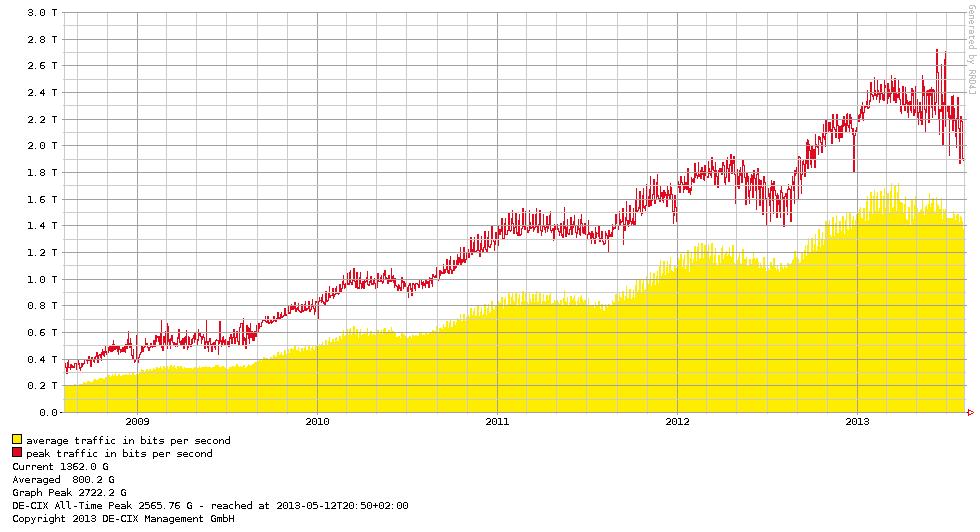
\includegraphics[keepaspectratio,width=0.9\textwidth]{abbildungen/de-cix_5y_20130804.png}
 \caption{DE-CIX Traffic Statistik, 5 Jahres Grafik \protect\footnotemark[1]}
 %\caption{DE-CIX traffic statistics, 5 year graph \protect\footnotemark[1]}
 \label{fig:DE-CIX}
\end{figure}

\footnotetext[1]{\url{http://www.de-cix.net/about/statistics/}}

Eine verständliche Einführung in die Tiefen der optischen Übertragungstechnik bietet das Vorlesungsskript OUET \cite{ouet}.
Eine weitere wichtigste Quellen ist \cite{Agrawal2012}.



\section{Abkürzungen}
Für Abkürzungen kann das Paket \textit{acronym} verwendet werden.
Ein Abkürzungsverzeichnis ist nicht erforderlich, sofern alle Akbürzungen bei der ersten Verwendung eingeführt werden.
Dies wird durch die Verwendung von \textit{acronym} vereinfacht, jedoch ist die Nutzung des Paketes rein optional.
Das Paket bietet folgende Optionen (siehe  \LaTeX~Quelltext):\par\medskip
\begin{itemize}
 \item \ac{NLSE}         % fügt die Abkürzung ein, außer beim ersten Aufruf, hier wird die Erklärung mit angefügt
 \item \acs{NLSE}        % fügt die Abkürzung ein
 \item \acf{NLSE}        % fügt die Abkürzung UND die Erklärung ein
 \item \acl{NLSE}        % fügt nur die Erklärung ein
\end{itemize}



\section{Mathematik}
Für mathematische Formeln wird das \textit{amsmath} Paket verwendet. Gleichungen sind damit recht schön zu setzen:

\begin{equation}
\frac{{\partial A}}{{\partial z}} =  - \frac{\alpha }{2}A + i{\beta ^{(0)}}A - {\beta ^{(1)}}\frac{{\partial A}}{{\partial t}} - i\frac{{{\beta ^{(2)}}}}{2}\frac{{{\partial ^2}A}}{{\partial {t^2}}} + i\gamma {\left| A \right|^2}A
\label{equ:nlse}
\end{equation}

Auch das Referenzieren von Gleichungen ist recht einfach. Dabei ist mit Gleichung \eqref{equ:nlse} eine mögliche Darstellungsform der \acs{NLSE} gegeben.

\fi
